\documentclass[internal]{../../classes/nervtech-research}

\nervsetup{
  company={NervTech},
  project={Node v0},
  document={Research Notes},
  subtitle={Problem framing, goal association, assumptions and associated research papers},
  docid={NT-N-M-H-001},
  revision={A},
  status={Exploratory Draft},
  author={NervTech Research},
  owner={Robotics Systems Engineering},
  date={2026-07-9},
  stage={Preliminary Research},
  question={Which motor housing architecture will fulfill NT-N-G1, NT-N-G2 and NT-N-G7?},
  keywords={integrated actuator, mechanical design, motor housing, robotics, research notes},
  abstract={This document collates and analyses multiple research papers and notes for fulfilling Node v0 design goals. Its intended purpose is to isolate observations, assumptions, risks, and design direction before committing to a detailed technical design.}
}

\begin{document}
\maketitle
\tableofcontents
\newpage

\section{Research Snapshot}
\researchsnapshot
{Build motor housing to maximise thermal and electromagnetic performance of the actuator, while reducing size and weight.}
{The highest leverage early decision is the actuator architecture, because it constrains torque density, controllability, thermal behaviour, and manufacturability.}
{The true operating envelope is still uncertain: load profile, duty cycle, heat rejection, encoder resolution, and gearbox backlash all need validation.}
{Prototype the smallest credible bench rig and measure torque, speed, temperature rise, backlash, and closed-loop response.}

\section{Problem Framing}
\begin{researchquestion}[System Direction]
  What outrunner BLDC motor housing architectures minimises thermal resistance (\textdegree C/W), magnetic flux leakage and Air Gap instability ($\pm$ mm)?
\end{researchquestion}

\section{Preliminary Direction}
This research document will collate results from multiple research papers and notes to inform the design of a motor housing for Node v0.
The goal is to identify the most promising motor housing architecture that meets the specified design goals (NT-N-G1, NT-N-G2, NT-N-G7).
A preliminary frameless outrunner BLDC motor has been selected, informed by cost and performance requirements.

\section{Assumptions}
\begin{itemize}
  \item The frameless outrunner BLDC architecture will provide the highest torque density and lowest thermal resistance for the Node v0 actuator.
  \item Aluminium provides the best balance of thermal conductivity, weight, and manufacturability for the motor housing.
\end{itemize}

\newpage

\section{Frameless BLDC Architecture}
The selected frameless outrunner BLDC was the SteadyWin WK8115 model with the following dimensions:
\begin{figure}[h!]
  \centering
  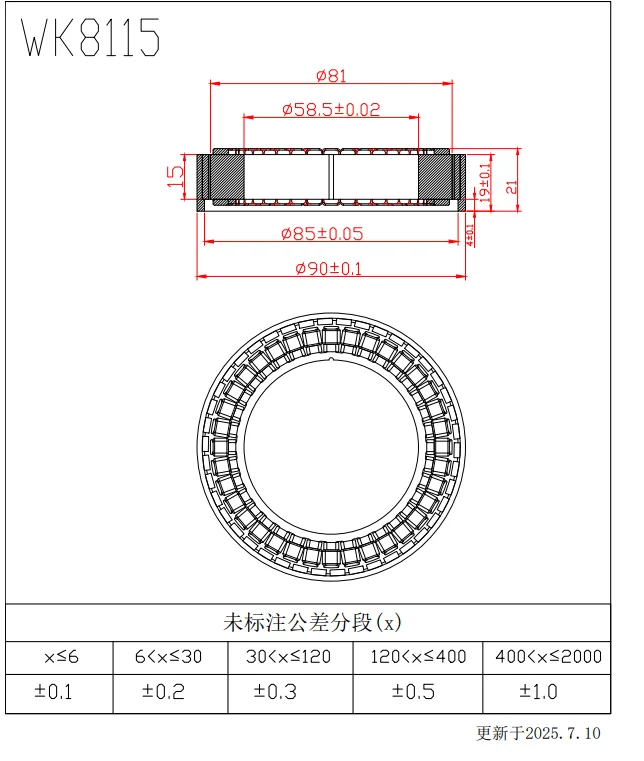
\includegraphics[width=0.8\textwidth]{figures/NT-N-P001.png}
  \caption{SteadyWin WK8115 Dimensions}
  \label{fig:wk8115_dimensions}
\end{figure}
\clearpage
The magnetic, thermal and electrical properties of the motor are taken from the manufacturer as follows:
\begin{figure}[h!]
  \centering
  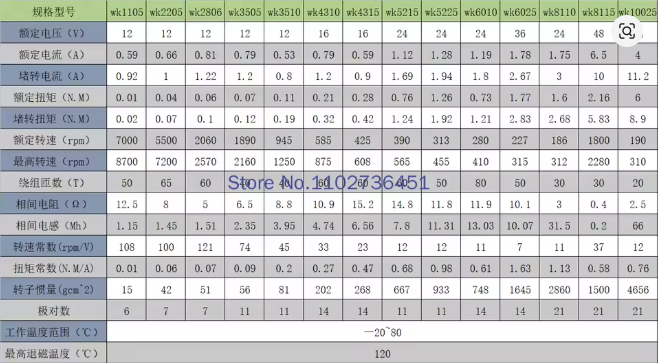
\includegraphics[width=0.8\textwidth]{figures/NT-N-P002.png}
  \caption{SteadyWin WK8115 Specifications}
  \label{fig:wk8115_specifications}
\end{figure}
\newline
Figure~\ref{fig:wk8115_dimensions} will inform the tolerances and mechanical design of the Node v0 motor housing, while Figure~\ref{fig:wk8115_specifications} will inform the thermal and electromagnetic characteristics of the Node v0 actuator.

\section{Kollmorgen Mounting and Installation Guidelines}
Kollmorgen is a German engineering company that provides a range of motion control solutions.
While the procured SteadyWin WK8115 is not a Kollmorgen product, the company provides a set of mounting and installation guidelines that can be applied to the Node v0 motor housing design.

\subsubsection{Bearings}
Bearings in the motor housing are critical for maintaining air gap stability and therefore electromagnetic performance \cite{KollmorgenManual}.
Kollmorgen notes that concentricity requirements are noted on the motor datasheet, and should be considered when "sizing and selecting bearings for appropriate radial and preload forces to achieve desired motor running gap clearance and total runout".
Bearings should also be chosen for the lowest possible friction and high quality lubricant, to reduce motor losses and heat generation.
Similar Kollmorgen outrunner BLDC motors to the WK8115 can be observed to find appropriate concentricity requirements, and a factor of safety can be applied to account for the lower quality of the SteadyWin motor.
\\\\
The Kollmorge


\clearpage

\begin{thebibliography}{9}

\bibitem{KollmorgenManual}
Kollmorgen Corporation (2020) \emph{Mounting and Installation Guidelines for BLDC Motors}, Kollmorgen Technical Documentation.

\bibitem{lamport94}
Leslie Lamport (1994) \emph{\LaTeX: a document preparation system}, Addison
Wesley, Massachusetts, 2nd ed.
\end{thebibliography}

\end{document}
